%!TEX program=xelatex
%!TEX spellcheck=en_US
\documentclass[final]{report}
% Include all project wide packages here.
%\usepackage{fullpage}
\usepackage[a4paper,margin=4cm,top=2cm,bottom=3cm]{geometry}
\usepackage{polyglossia}
\setmainlanguage{english}
\usepackage{csquotes}
\usepackage{graphicx}
\usepackage{pdfpages}
\usepackage{caption}
\usepackage[list=true]{subcaption}
\usepackage{float}
\usepackage{standalone}
\usepackage{import}
\usepackage{tocloft}
\usepackage{wrapfig}
\usepackage{authblk}
\usepackage{array}
\usepackage{booktabs}
\usepackage[title,titletoc]{appendix}
\usepackage{fontspec}
\usepackage{pgfplots}
\usepackage{tikz}
\usepackage[binary-units=true,parse-numbers=true,table-auto-round=true]{siunitx}
\DeclareSIUnit\flops{FLOPS}
\DeclareSIUnit\iops{IOPS}
\sisetup{detect-weight=true}
\usepackage{units}
\usepackage{amsmath}
\usepackage{mathtools}
\usepackage{unicode-math}
\usepackage{rotating}
\usepackage[compact]{titlesec}
\usepackage{titletoc}
\usepackage{blindtext}
\usepackage{color}
\usepackage{enumitem}
\usepackage{tabularx}
\usepackage{titling}
\usepackage[%
siunitx,
fulldiodes,
europeanvoltages,
europeancurrents,
europeanresistors,
americaninductors,
smartlabels]{circuitikz}

\usetikzlibrary{calc}
\usetikzlibrary{positioning}
\usetikzlibrary{automata}
\usetikzlibrary{arrows.meta}

\tikzstyle{every state}=[fill=tu-cyan,align=center,draw=black,line width=1pt,node distance=3cm,minimum width = 1.8cm]%for FSMs casper
\tikzstyle{every initial by arrow}=[initial text={Reset}]
\newcommand{\setpathasarrows}{\tikzstyle{every path}=[auto,line width=1.5pt,line cap=round,line join=round]}

\pgfplotsset{compat=newest}
\pgfplotsset{plot coordinates/math parser=false}
\usetikzlibrary{plotmarks}
\usepgfplotslibrary{patchplots}
\newlength\figureheight
\newlength\figurewidth

\usepackage[
%backend=bibtex,
backend=biber,
	texencoding=utf8,
bibencoding=utf8,
style=numeric,
citestyle=numeric,
    sortlocale=en_US,
    language=auto,
    backref=true,
    abbreviate=false,
    date=iso8601
]{biblatex}


\usepackage{listings}
\newcommand{\includecode}[4][c]{\lstinputlisting[caption=#2, escapechar=, style=#1,label=#4]{#3}}
\newcommand{\superscript}[1]{\ensuremath{^{\textrm{#1}}}}
\newcommand{\subscript}[1]{\ensuremath{_{\textrm{#1}}}}


\newcommand{\chapternumber}{\thechapter}
\renewcommand{\appendixname}{Appendix}
\renewcommand{\appendixtocname}{Appendices}
\renewcommand{\appendixpagename}{Appendices}


\setlist[enumerate]{labelsep=*, leftmargin=1.5pc}
\setlist[enumerate,1]{label=\arabic*., ref=\arabic*}
\setlist[enumerate,2]{label=\arabic*.,ref=\theenumi.\arabic*}
\setlist[enumerate,3]{label=\arabic*., ref=\theenumii.\arabic*}

\usepackage{xr-hyper}
\usepackage[hidelinks]{hyperref} %<--------ALTIJD ALS LAATSTE
\usepackage[nameinlink,noabbrev,capitalise]{cleveref} %<------- Clever Ref moet na hyperref
\crefname{app}{Appendix}{Appendices}
%\renewcommand{\familydefault}{\sfdefault}


\setmainfont{Myriad Pro}[Ligatures={Common,TeX}]
%\setmathfont{Asana Math}
\setmathfont{Asana-Math.otf}
\setmonofont[Scale=0.9]{Lucida Console}
\newfontfamily\headingfont{Minion Pro}[Ligatures={Common,TeX}]


%Design colors
\definecolor{accent1}{RGB}{0,100,200}
\definecolor{accent2}{RGB}{0,50,100}
\definecolor{tu-cyan}{RGB}{0,166,214}

\newcommand{\hsp}{\hspace{20pt}}
\titleformat{\chapter}[hang]{\Huge\headingfont}{\chapternumber\hsp\textcolor{accent2}{|}\hsp}{0pt}{\Huge\headingfont}

\titleformat{name=\chapter,numberless}[hang]{\Huge\headingfont}{\hsp\textcolor{accent2}{|}\hsp}{0pt}{\Huge\headingfont}

\titleformat{\section}[block]{\LARGE\headingfont}{\arabic{chapter}.\arabic{section}}{0.4em}{}
\titleformat{\subsection}[block]{\Large\headingfont}{\arabic{chapter}.\arabic{section}.\arabic{subsection}}{0.4em}{}
\titleformat{\subsubsection}[block]{\large\headingfont}{\arabic{chapter}.\arabic{section}.\arabic{subsection}.\arabic{subsubsection}}{0.4em}{}
\renewcommand{\arraystretch}{1.25}
\renewcommand{\baselinestretch}{1.25}

\renewcommand\cfttoctitlefont{\headingfont\Huge}
\renewcommand\cftloftitlefont{\headingfont\Huge}
\renewcommand\cftlottitlefont{\headingfont\Huge}
\setcounter{lofdepth}{2}
\setcounter{lotdepth}{2}


\setlength{\parindent}{0pt}
\setlength{\parskip}{0.75em}


%SIuntix settings:
%default: 0V to 10V
%custom: 0 - 10V
\sisetup{range-phrase=--}
\sisetup{range-units=single}
\DeclareSIUnit\years{years}

%For code listings
\definecolor{black}{rgb}{0,0,0}
\definecolor{browntags}{rgb}{0.65,0.1,0.1}
\definecolor{bluestrings}{rgb}{0,0,1}
\definecolor{graycomments}{rgb}{0.4,0.4,0.4}
\definecolor{redkeywords}{rgb}{1,0,0}
\definecolor{bluekeywords}{rgb}{0.13,0.13,0.8}
\definecolor{greencomments}{rgb}{0,0.5,0}
\definecolor{redstrings}{rgb}{0.9,0,0}
\definecolor{purpleidentifiers}{rgb}{0.01,0,0.01}


\lstdefinestyle{csharp}{
language=[Sharp]C,
showspaces=false,
showtabs=false,
breaklines=true,
showstringspaces=false,
breakatwhitespace=true,
escapeinside={(*@}{@*)},
columns=fullflexible,
commentstyle=\color{greencomments},
keywordstyle=\color{bluekeywords}\bfseries,
stringstyle=\color{redstrings},
identifierstyle=\color{purpleidentifiers},
basicstyle=\ttfamily\small}

\lstdefinestyle{c}{
language=C,
showspaces=false,
showtabs=false,
breaklines=true,
showstringspaces=false,
breakatwhitespace=true,
escapeinside={(*@}{@*)},
columns=fullflexible,
commentstyle=\color{greencomments},
keywordstyle=\color{bluekeywords}\bfseries,
stringstyle=\color{redstrings},
identifierstyle=\color{purpleidentifiers},
}

\lstdefinestyle{cpp}{
language=C++,
showspaces=false,
showtabs=false,
breaklines=true,
showstringspaces=false,
breakatwhitespace=true,
escapeinside={(*@}{@*)},
columns=fullflexible,
commentstyle=\color{greencomments},
keywordstyle=\color{bluekeywords}\bfseries,
stringstyle=\color{redstrings},
identifierstyle=\color{purpleidentifiers},
}

\lstdefinestyle{matlab}{
language=Matlab,
showspaces=false,
showtabs=false,
breaklines=true,
showstringspaces=false,
breakatwhitespace=true,
escapeinside={(*@}{@*)},
columns=fullflexible,
commentstyle=\color{greencomments},
keywordstyle=\color{bluekeywords}\bfseries,
stringstyle=\color{redstrings},
identifierstyle=\color{purpleidentifiers}
}

\lstdefinestyle{vhdl}{
language=VHDL,
showspaces=false,
showtabs=false,
breaklines=true,
showstringspaces=false,
breakatwhitespace=true,
escapeinside={(*@}{@*)},
columns=fullflexible,
commentstyle=\color{greencomments},
keywordstyle=\color{bluekeywords}\bfseries,
stringstyle=\color{redstrings},
identifierstyle=\color{purpleidentifiers}
}

\lstdefinestyle{xaml}{
language=XML,
showspaces=false,
showtabs=false,
breaklines=true,
showstringspaces=false,
breakatwhitespace=true,
escapeinside={(*@}{@*)},
columns=fullflexible,
commentstyle=\color{greencomments},
keywordstyle=\color{redkeywords},
stringstyle=\color{bluestrings},
tagstyle=\color{browntags},
morestring=[b]",
  morecomment=[s]{<?}{?>},
  morekeywords={xmlns,version,typex:AsyncRecords,x:Arguments,x:Boolean,x:Byte,x:Char,x:Class,x:ClassAttributes,x:ClassModifier,x:Code,x:ConnectionId,x:Decimal,x:Double,x:FactoryMethod,x:FieldModifier,x:Int16,x:Int32,x:Int64,x:Key,x:Members,x:Name,x:Object,x:Property,x:Shared,x:Single,x:String,x:Subclass,x:SynchronousMode,x:TimeSpan,x:TypeArguments,x:Uid,x:Uri,x:XData,Grid.Column,Grid.ColumnSpan,Click,ClipToBounds,Content,DropDownOpened,FontSize,Foreground,Header,Height,HorizontalAlignment,HorizontalContentAlignment,IsCancel,IsDefault,IsEnabled,IsSelected,Margin,MinHeight,MinWidth,Padding,SnapsToDevicePixels,Target,TextWrapping,Title,VerticalAlignment,VerticalContentAlignment,Width,WindowStartupLocation,Binding,Mode,OneWay,xmlns:x}
}

\lstdefinestyle{python}{
language=Python,
showspaces=false,
showtabs=false,
breaklines=true,
showstringspaces=false,
breakatwhitespace=true,
escapeinside={(*@}{@*)},
columns=fullflexible,
commentstyle=\color{greencomments},
keywordstyle=\color{bluekeywords}\bfseries,
stringstyle=\color{redstrings},
identifierstyle=\color{purpleidentifiers},
}

%defaults
\lstset{
basicstyle=\ttfamily\scriptsize ,
extendedchars=false,
numbers=left,
numberstyle=\ttfamily\tiny,
stepnumber=1,
tabsize=4,
numbersep=5pt
}
\addbibresource{../../.library/bibliography.bib}
\begin{document}
\chapter{OpenMP}
%TODO OpenMP Test Number of threads. DP and SP.
\section{Task 1}
In order to find the most suitable number of threads a fixed data size of 2048 bytes with a sweep from 1 to 64 threads has been used.
\begin{figure}[H]
\centering
    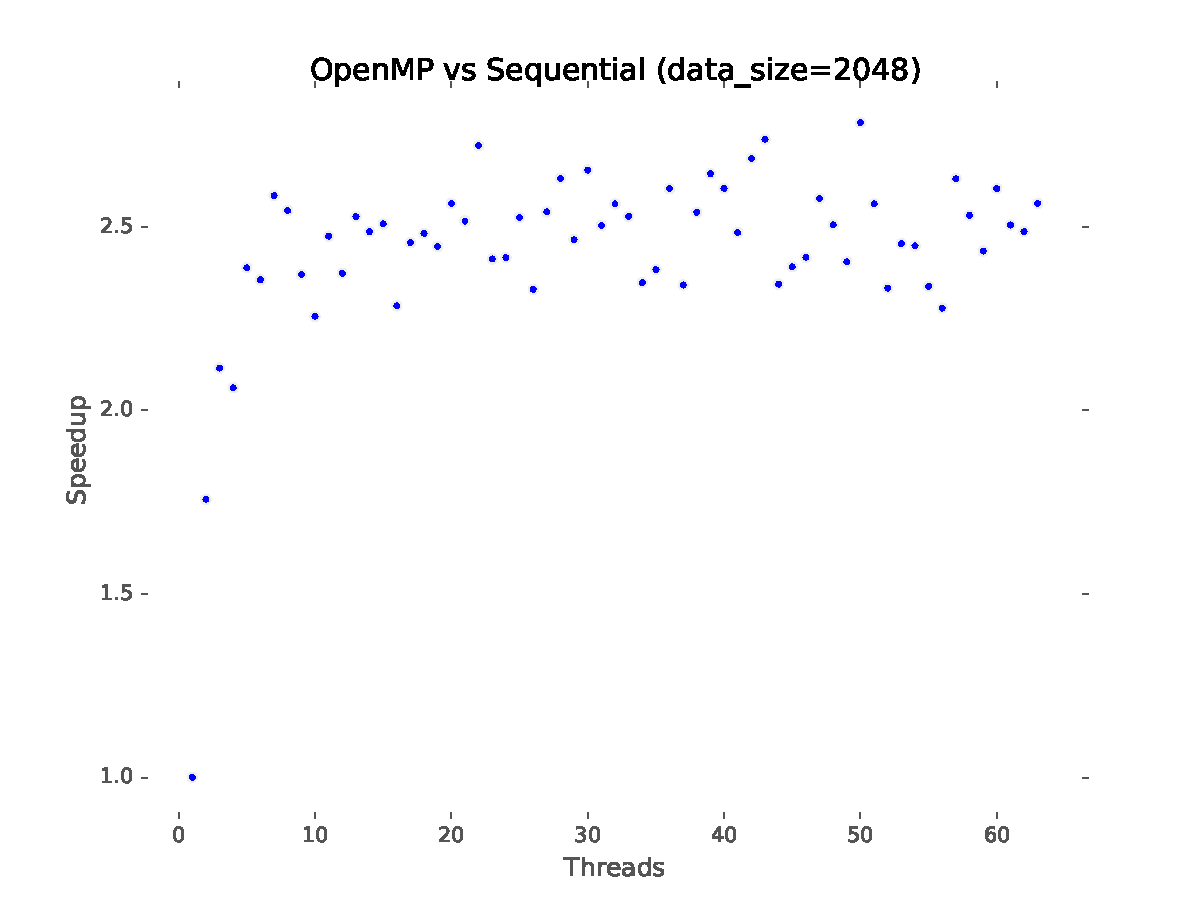
\includegraphics[width=\linewidth]{resources/openmp-number-of-threads-sweep.pdf}
    \caption{The speedup of the OpenMP version with varying threads, uses a data\_size of 2048.}
    \label{fig:openmp-number-of-threads-sweep}
\end{figure}
Looking at \autoref{fig:openmp-number-of-threads-sweep}, the first thing that comes to mind is the sharp inclination in speedup till 8 threads after which the speedup basically stalls.

The initial increase in speedup is obvious, the program is able to perform parallel computations and every thread addition, up to a certain point, contributes to the speedup.

The reason that the speedup growth is slowing down is because of two things.
Firstly, the execution time of the sequential part of the program is getting bigger compared to that of the parallel part.
Secondly, the machine that this code is running on has 8 virtual cores with hyperthreading enabled.
This is likely the cause why after 8 threads the extra amount of threads are just polluting the cores and not really using extra compute power.

Another note can be made about the 3th-4th, 5th-6th and the 7th-8th number of threads.
Here the 4th, 6th and 8th number of threads seem not to be contributing to the speedup, on the contrary they even cause a slight bump in speedup.
The reason for this stays unclear and is beyond the scope of this report.

\section{Task 2}
Taken from the previous task, the most suitable number of threads seems to lay between 8-64 threads.
Since, 50 threads gave the biggest speedup improvement, this amount of threads will be used for this task; it is however highly influenced by a lot of factors and this number changes everytime you run the application.

%TODO OpenMP Test Data Size. DP and SP.
\begin{figure}[H]
\centering
    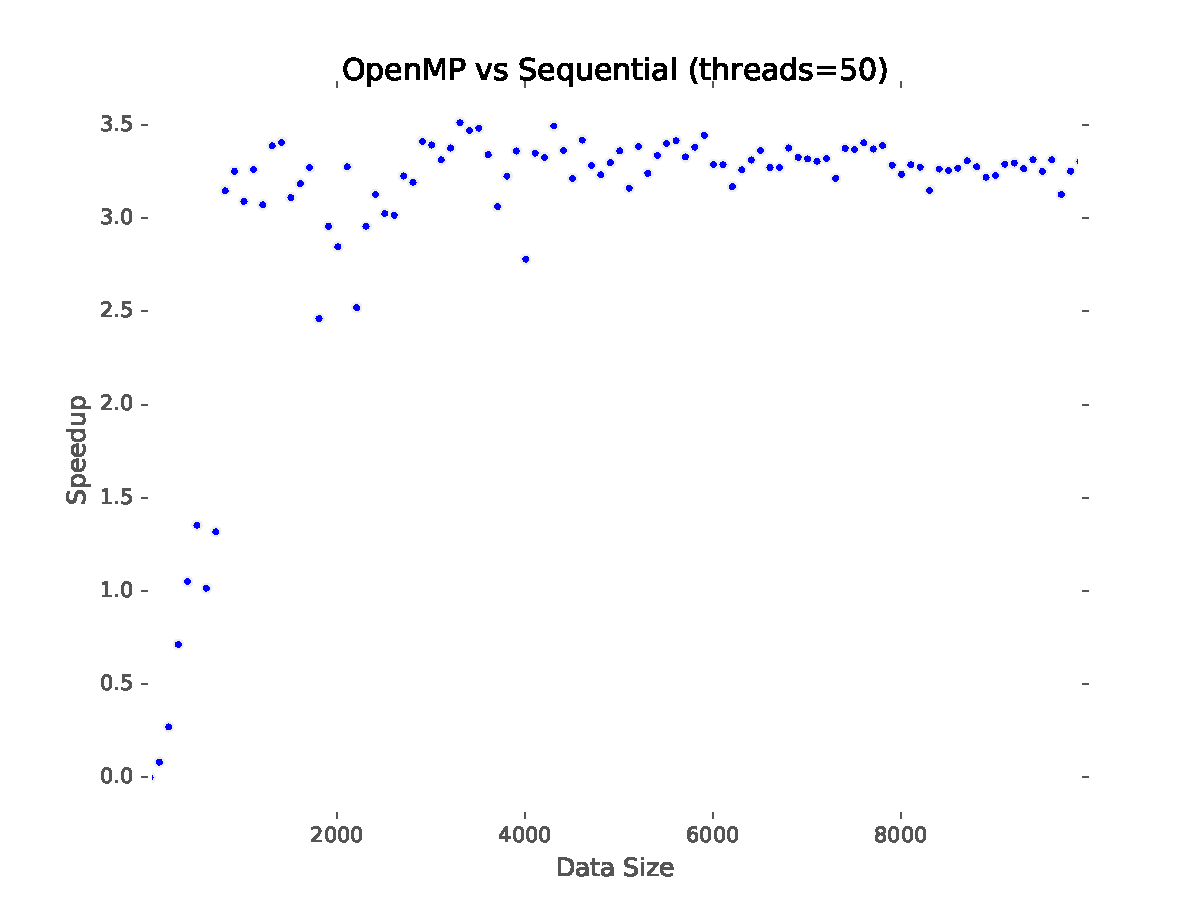
\includegraphics[width=\linewidth]{resources/openmp-data-size-sweep.pdf}
    \caption{The speedup of the OpenMP version with varying data\_size, uses 50 threads.}
    \label{fig:openmp-data-size-sweep}
\end{figure}

For small data sizes one can see that the speedup is below one.
This is caused due to the overhead caused by starting and managing multiple threads, while they are not very beneficial yet for the application.
The computation time is relatively short compared to the startup time for these smaller data sizes. For bigger data sizes one can see a sharp inclination in speedup till the 1000 data size mark is reached, after this the speedup seems to stall around 3.3.

Another thing that can be noticed is that the data becomes less noisy towards the end of the graph, for bigger data sizes that is.
This is likely caused by the computational part of the program getting bigger, causing other system parameters to have influence on the overall running time.

In \cref{lst:openmp-matrix-snippet} our matrix OpenMP code is shown, the inner loop is added to sum over all rows of the first matrix.
\includecode[cpp]{OpenMP Matrix x Matrix Snippet}{resources/OpenMPMatrixSnippet.cpp}{lst:openmp-matrix-snippet}

\end{document}